\documentclass[a4paper]{article}

\usepackage[utf8]{inputenc}
\usepackage{lmodern}
\usepackage[T1]{fontenc}
\usepackage[babel=true]{microtype}
\usepackage[portuguese]{babel}
\usepackage[pdftex]{hyperref}
\usepackage{graphicx}
\usepackage{eurosym}
\usepackage{scrextend}
\usepackage{hyphenat}
\usepackage{url}
\usepackage{hyperref}
\usepackage{float}
\usepackage{indentfirst}
\usepackage{verbatim}
\usepackage{listings}
\usepackage[usenames,dvipsnames,svgnames,table]{xcolor}

\lstdefinestyle{customprolog}{
  belowcaptionskip=1\baselineskip,
  breaklines=true,
  xleftmargin=\parindent,
  language=Prolog,
  showstringspaces=false,
  tabsize=2,
  basicstyle=\footnotesize\ttfamily,
  keywordstyle=\bfseries\color{blue},
  commentstyle=\itshape\color{gray},
  identifierstyle=\color{black},
  stringstyle=\color{OliveGreen},
}

\lstdefinestyle{customprologwithlines}{
  belowcaptionskip=1\baselineskip,
  breaklines=true,
  xleftmargin=\parindent,
  language=Prolog,
  showstringspaces=false,
  tabsize=2,
  numbers=left,
  basicstyle=\footnotesize\ttfamily,
  keywordstyle=\bfseries\color{blue},
  commentstyle=\itshape\color{gray},
  identifierstyle=\color{black},
  stringstyle=\color{OliveGreen},
}

\begin{document}

\setlength{\textwidth}{16cm}
\setlength{\textheight}{22cm}

\title{\Huge\textbf{Jogo Cage}\linebreak\linebreak\linebreak
\Large\textbf{Relatório Final}\linebreak\linebreak
\linebreak\linebreak

\includegraphics[scale=0.1]{resources/feup-logo.png}\linebreak\linebreak
\linebreak\linebreak
\Large{Mestrado Integrado em Engenharia Informática e Computação} \linebreak\linebreak
\Large{Programação em Lógica}\linebreak
}

\author{\textbf{Grupo 2:}\\ José Peixoto - 200603103 \\ Luís Cruz - 201303248 \\\linebreak\linebreak \\
 \\ Faculdade de Engenharia da Universidade do Porto \\ Rua Roberto Frias, s\/n, 4200-465 Porto, Portugal \linebreak\linebreak\linebreak
\linebreak\linebreak\vspace{1cm}}
%\date{Junho de 2007}
\maketitle
\thispagestyle{empty}

%************************************************************************************************
%************************************************************************************************

\newpage

\section*{Resumo}
No âmbito da unidade curricular de Programação em Lógica, foi-nos proposto o desenvolvimento de um jogo de tabuleiro em \emph{Prolog}: o \emph{Cage}. O principal objetivo na realização deste projeto foi a aquisição de novas competências na expressão de conceitos lógicos em \emph{Prolog}. Abordámos o problema de forma iterativa, tendo feito numa primeira fase, um levantamento das regras do jogo e posteriormente uma reflexão sobre a representação do estado do jogo. Uma vez implementados os procedimentos para uma manipulação básica de listas, iniciámos o desenvolvimento da interface de linha de comandos básica e posteriormente, um modo de jogo humano contra humano básico, para o qual se tentou adicionar e testar as jogadas previstas para o jogo. Numa fase final implementou-se um modo de jogo automático no qual é feita uma seleção aleatória de jogadas válidas.   

Findo o projeto, realçamos a vantagem na expressividade do \emph{Prolog} em conceitos lógicos, e a nossa carência de experiência com este paradigma de programação.

\newpage

\tableofcontents

%************************************************************************************************
%************************************************************************************************

%*************************************************************************************************
%************************************************************************************************

\newpage

%%%%%%%%%%%%%%%%%%%%%%%%%%
\section{Introdução}

O principal objetivo na realização deste projeto foi a aquisição de novas competências na expressão de conceitos lógicos em \emph{Prolog} ao implementar uma versão do jogo de tabuleiro \emph{Cage}. Este relatório tenta explicar o estado final do projeto, salientando as suas funcionalidades e incluindo imagens ilustrativas do resultado final.

%%%%%%%%%%%%%%%%%%%%%%%%%%
\section{O Jogo Cage}
O Cage é um jogo de estratégia em tabuleiro semelhante às damas que foi inventado por Mark Steere em maio de 2010. O autor descreve-o como um jogo para dois jogadores sem qualquer informação oculta. É um jogo abstrato sem fator de sorte nem empates. É jogado num tabuleiro de damas 10x10 ou 8x8 e, ao contrário do jogo original das damas, todo tabuleiro está preenchido, no início, com peças já promovidas a ``damas''. ``Jogo de aniquilação de alta energia'' é a frase escolhida pelo autor para caricaturar o jogo, uma vez que o movimento para o centro do tabuleiro assegura a aniquilação, de pelo menos, uma das cores.

\subsection{Regras}
O Cage é jogado por dois jogadores num tabuleiro de damas com 50 damas vermelhas e 50 damas azuis na versão de tabuleiro 10x10 ou com 32 damas vermelhas e 32 damas azuis na versão de 8x8 tabuleiro. O tabuleiro é iniciado preenchendo todas as casas com damas de cor alternada.

\subsubsection{Objetivo}
Para vencer é necessário capturar todas as damas inimigas. No final, pode ganhar-se mesmo que se perca a última peça que se está a movimentar (saltar) para capturar todas as damas inimigas ainda em jogo.

\subsubsection{Movimentos}
Existem quatro tipos de movimentos:
\begin{enumerate}
  \item Restrito
  \item Centralizador
  \item Adjacente
  \item Salto
\end{enumerate}
Durante um turno, um jogador apenas pode utilizar um tipo de movimento.

\paragraph{Restrição 1}
Nunca se pode colocar uma dama ortogonalmente (horizontal ou verticalmente) adjacente a uma dama de cor idêntica. Nem de forma transitória durante um turno de vários movimentos.

\paragraph{Restrição 2}
Nunca se pode movimentar uma dama que tenha adjacências ortogonais com damas inimigas para uma casa onde tal não aconteça.

\paragraph{Centralizador}
Este movimento de uma casa, permite à dama deslocar-se na horizontal, vertical ou diagonal para uma casa vazia e que permite que a dama se aproxime do centro do tabuleiro.

\paragraph{Adjacente}
Uma dama que não tenha adjacências ortogonais com damas inimigas pode mover-se apenas uma casa em qualquer direção que contenha adjacências ortogonais com uma ou mais damas inimigas.

\paragraph{Salto}
O movimento de salto permite capturar uma dama inimiga, movimentando a dama do jogador de uma casa ortogonalmente adjacente de um lado da dama inimiga para a casa vazia adjacente do lado oposto. É possível capturar uma dama inimiga nas casas periféricas do tabuleiro de uma casa adjacente e do lado oposto da dama inimiga na borda do tabuleiro. O resultado é que quer a dama capturada quer a dama que captura são removidas do tabuleiro.

%%%%%%%%%%%%%%%%%%%%%%%%%%
\section{Lógica do Jogo}

\subsection{Representação do Estado do Jogo} 
Na representação do tabuleiro de jogo usam-se listas de listas que apenas incluem
átomos para os diferentes tipos de peças ($red$ e $blue$) e a casa vazia ($empty$). Para simplificação do desenvolvimento do jogo, escolheu-se a versão mais pequena do tabuleiro 8x8 com um total de 64 damas no início do jogo. O tabuleiro por sua vez é um elemento de uma lista que contém, além do tabuleiro, informação relativa ao estado do jogo, como o número de peças vermelhas e azuis, o modo de jogo, a situação de obrigação de salto e as coordenadas de uma posição da qual um salto é obrigatório.
 
\subsubsection{Representação do estado inicial do tabuleiro:}
\begin{verbatim}
[[blue,red,blue,red,blue,red,blue,red],
 [red,blue,red,blue,red,blue,red,blue],
 [blue,red,blue,red,blue,red,blue,red],
 [red,blue,red,blue,red,blue,red,blue],
 [blue,red,blue,red,blue,red,blue,red],
 [red,blue,red,blue,red,blue,red,blue],
 [blue,red,blue,red,blue,red,blue,red],
 [red,blue,red,blue,red,blue,red,blue]
]).
\end{verbatim}

\begin{figure}[H]
    \center
    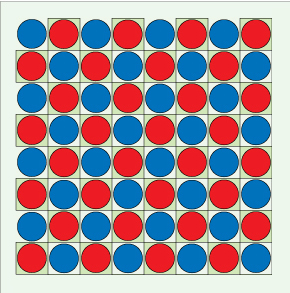
\includegraphics[scale=0.4]{resources/initial-state.jpg}
    \caption{Estado inicial do jogo}
    \label{fig:initial-state.png}
\end{figure}

\subsection{Visualização do Tabuleiro}

O tabuleiro pode ser visualizado pela linha de comandos a cada nova jogada efetuada quer pelo utilizador quer pelo computador.
É disponibilizada informação acerca das peças ainda em jogo, e auxiliares na seleção de jogadas como a letra representativa de uma coluna e um número para uma linha.

\begin{figure}[H]
    \center
    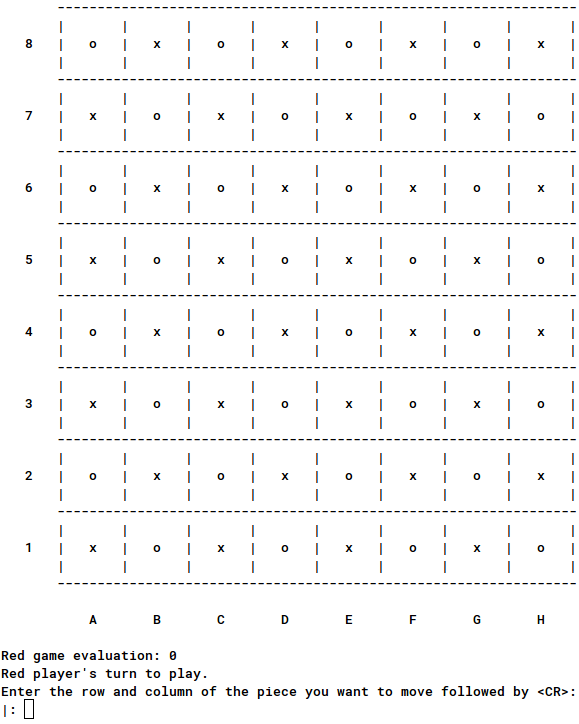
\includegraphics[scale=0.5]{resources/piece-selection.png}
    \caption{Estado inicial do jogo com pedido de seleção de jogada}
    \label{fig:piece-selection.png}
\end{figure}

\subsection{Lista de Jogadas Válidas}
Não está implementado nenhum método que angarie um conjunto de jogadas válidas, no entanto é possível determinar se existem movimentos válidos para uma dada peça do tabuleiro, sem movimentar nenhuma peça do tabuleiro, através de uma chamada à função \texttt{check\_move\_availability}.

\begin{lstlisting}[style=customprolog]
check_move_availability(SrcRow, SrcCol, Player, Board):-
	% a move must be checked in all directions
	IncRow is SrcRow + 1,
	DecRow is SrcRow - 1,
	IncCol is SrcCol + 1,
	DecCol is SrcCol - 1,
	(
	   IncRow =< 7, validate_move(SrcRow, SrcCol, IncRow, SrcCol, Player, Board, _, _);
	   DecRow >= 0, validate_move(SrcRow, SrcCol, DecRow, SrcCol, Player, Board, _, _);
	   IncCol =< 7, validate_move(SrcRow, SrcCol, SrcRow, IncCol, Player, Board, _, _);
	   DecCol >= 0, validate_move(SrcRow, SrcCol, SrcRow, DecCol, Player, Board, _, _);
	   DecRow >= 0, DecCol >= 0, validate_move(SrcRow, SrcCol, DecRow, DecCol, Player, Board, _, _);
	   IncRow =< 7, IncCol =< 7, validate_move(SrcRow, SrcCol, IncRow, IncCol, Player, Board, _, _);
	   DecRow >= 0, IncCol =< 7, validate_move(SrcRow, SrcCol, DecRow, IncCol, Player, Board, _, _);
	   IncRow =< 7, DecCol >= 0, validate_move(SrcRow, SrcCol, IncRow, DecCol, Player, Board, _, _)
	), !.
\end{lstlisting}

\subsection{Execução de Jogadas}
No caso da seleção de uma jogada manualmente através da consola, com a introdução de uma letra a representar a coluna e um número a representar uma linha, o programa tenta validar e mover uma peça do tabuleiro, tentando primeiro fazer uma jogada do tipo de salto. Quando o salto falha, são tentados outros dois tipos de movimentos: um adjacente e por fim, em último recurso, um movimento centralizador. Caso nenhum movimento seja válido, de acordo com as regras, assume-se que o jogador tem de dar a vez ao seu adversário. Em nenhum caso o jogo pode ficar numa situação na qual nenhum dos dois jogadores está sem jogadas válidas para executar.

\begin{lstlisting}[style=customprolog]
make_move(SrcRow,SrcCol, DestRow, DestCol, Game, ModifiedGame):-
	(       
	   nl, write('Attempting to make a jump move...'), nl,
	   make_jump(SrcRow,SrcCol, DestRow, DestCol, Game, TemporaryGame);
	
	   write('Failed to make a jump move!'), nl, nl,
	   write('Attempting to make an adjoining move...'), nl,
	   make_adjoining_move(SrcRow,SrcCol, DestRow, DestCol, Game, TemporaryGame);
	
	   write('Failed to make an adjoining move!'), nl, nl,
	   write('Attempting to make a centering move...'), nl,
	   make_centering_move(SrcRow,SrcCol, DestRow, DestCol, Game, TemporaryGame);
	
	   write('Failed to make a centering move!'), nl, nl,
	   get_board(Game, Board), get_player_turn(Game, Player),
	   check_move_availability(SrcRow, SrcCol, Player, Board), ModifiedGame = Game;
	
	   write('No valid moves were available -> Switching player turn!'), nl, nl,
	   change_player_turn(Game,ModifiedGame), true
	),
get_force_jump(TemporaryGame, ForceJumpMode),
(
   ForceJumpMode == noForceJump -> change_player_turn(TemporaryGame,ModifiedGame),! ;
   ModifiedGame = TemporaryGame
).
\end{lstlisting}

\subsection{Avaliação do Tabuleiro}
Apesar de ser feita uma avaliação simples do estado do jogo, não é feito nenhum aproveitamento para além da visualização deste valor no início de cada jogada. É feito um cálculo da avaliação do tabuleiro para um dado jogador, com a diferença do seu número de peças com o número de peças do adversário. Neste jogo em específico, é um cálculo relativamente acertado, ignorando os casos em que, no turno em vigor é possível fazer múltiplos saltos, sendo a avaliação um valor subestimado.

\begin{lstlisting}[style=customprolog]
get_evaluation(Game,Player,Evaluation):-
    get_num_red_pieces(Game, NumRedPieces),
    get_num_blue_pieces(Game, NumBluePieces),
    (
       Player == redPlayer -> Evaluation is NumRedPieces - NumBluePieces;
       Player == bluePlayer -> Evaluation is NumBluePieces - NumRedPieces
    ),!.
\end{lstlisting} 

\subsection{Final do Jogo}
No início de cada iteração do ciclo principal do jogo, é feita a verificação do número de peças no tabuleiro. Quando um ou mais jogadores tiver zero peças em cima do tabuleiro o jogo está terminado e o vencedor foi o último jogador que fez uma movimentação no tabuleiro. É de salientar a possibilidade de o tabuleiro final estar completamente vazio, sendo o vencedor aquele que fez o salto final e que eliminou uma peça inimiga para fora do tabuleiro.

\begin{lstlisting}[style=customprolog]
validate_board_pieces(Game):-
    get_num_red_pieces(Game,NumRedPieces),
    get_num_blue_pieces(Game,NumBluePieces),
    NumRedPieces > 0,
    NumBluePieces > 0,!.
\end{lstlisting}

\begin{figure}[H]
    \center
    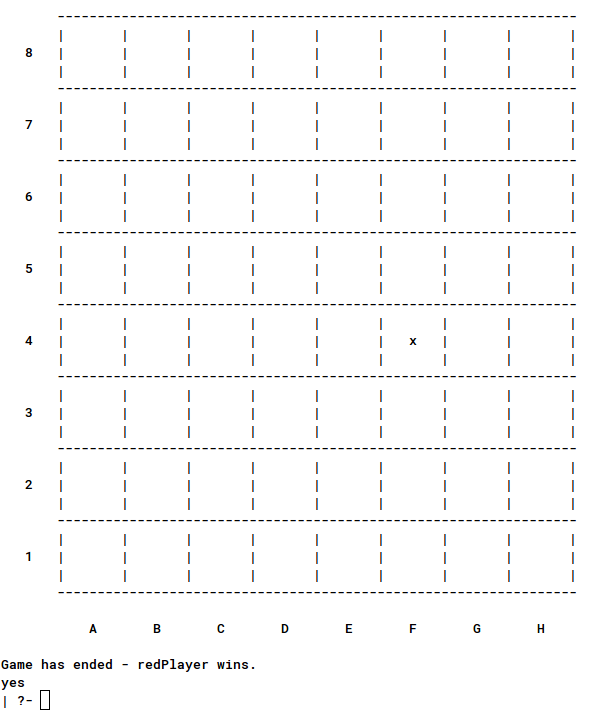
\includegraphics[scale=0.5]{resources/game-ending.png}
    \caption{Estado final de um jogo com declaração de vencedor}
    \label{fig:game-ending.png}
\end{figure}

\subsection{Jogada do Computador}
Não está implementada a possibilidade de seleção do modo de dificuldade de uma jogada do computador. O computador executa jogadas de forma aleatória.

%%%%%%%%%%%%%%%%%%%%%%%%%%
\section{Interface com o Utilizador}
No primeiro contato que o utilizador tem com o programa é-lhe solicitado o modo de jogo de três à disposição: humano contra humano, humano contra computador e computador contra computador.

\begin{figure}[H]
    \center
    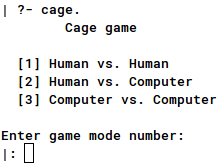
\includegraphics[scale=0.6]{resources/main-menu.png}
    \caption{Menu inicial do jogo}
    \label{fig:main-menu.png}
\end{figure}

A partir do momento em que o utilizador escolhe o modo de jogo computador contra computador, o programa inicia e finaliza rapidamente um jogo cujos movimentos são escolhidos pela simulação e execução aleatória de jogadas de forma automática. Nos outros dois modos de jogo, pode ser pedida a introdução de uma jogada a efectuar, contendo as coordenadas de partida e de destino de uma peça da cor do jogador do turno. Para tal usa-se a representação das coordenadas sob forma de uma letra de coluna seguido de um número da linha (Exemplo: $a2$ indica a coordenada de uma peça que está simultâneamente na coluna A e na linha 2). 

%%%%%%%%%%%%%%%%%%%%%%%%%%
\section{Conclusões}
Após a realização deste projeto, concluímos que ainda temos pouca experiência no desenvolvimento de procedimentos em programação em lógica e que muitos dos hábitos herdados de programação de outras linguagens nos trouxeram muitas situações ante problemas dos quais ainda não sabemos como contornar. É também de criticar a complexidade exagerada do trabalho, considerando o nosso conhecimento limitado e inexperiência na linguagem em questão, sendo que propomos este nível de complexidade apenas a partir de um segundo trabalho, ou um prazo de entrega mais alargado para este primeiro projeto.

\begin{thebibliography}{9}
\bibitem{lamport93}
  Sterling, Leon
  \emph{The Art of Prolog},
  The MIT Press
  2nd edition,
  2000.
  
  \bibitem{bl}Abstract games,
  \url{http://www.marksteeregames.com/MSG_abstract_games.html}, 14 10 2016.
  
  \bibitem{bl}Cage rules,
  \url{http://www.marksteeregames.com/Cage_rules.html}, 14 10 2016.
\end{thebibliography}

\newpage
\appendix
\section{Código fonte}
\subsection{board.pl}
\begin{lstlisting}[style=customprologwithlines]
% cell contents
cell(red).
cell(blue).
cell(empty).

% symbols
symbol(red,'x').
symbol(blue,'o').
symbol(empty,' ').

get_cell_symbol(empty,' ').
get_cell_symbol(red,'x').
get_cell_symbol(blue,'o').

piece_owned_by(red,redPlayer).
piece_owned_by(blue,bluePlayer).

get_board_cell(0,Col,[HeadList|_],Symbol):-
        get_list_element(Col,HeadList,Symbol).

get_board_cell(Row,Col,[_|TailList], Symbol):-
        Row > 0,
        Row1 is Row - 1,
        get_board_cell(Row1,Col,TailList,Symbol).

% checks if both players have pieces on the board
validate_board_pieces(Game):-
        get_num_red_pieces(Game,NumRedPieces),
        get_num_blue_pieces(Game,NumBluePieces),
        NumRedPieces > 0,
        NumBluePieces > 0,!.

% container | 32 red | 32 blue |
initial_board([[blue,red,blue,red,blue,red,blue,red],
               [red,blue,red,blue,red,blue,red,blue],
               [blue,red,blue,red,blue,red,blue,red],
               [red,blue,red,blue,red,blue,red,blue],
               [blue,red,blue,red,blue,red,blue,red],
               [red,blue,red,blue,red,blue,red,blue],
               [blue,red,blue,red,blue,red,blue,red],
               [red,blue,red,blue,red,blue,red,blue]
              ]).

% empty board | 0 red | 0 blue |
empty_board([[empty,empty,empty,empty,empty,empty,empty,empty],
             [empty,empty,empty,empty,empty,empty,empty,empty],
             [empty,empty,empty,empty,empty,empty,empty,empty],
             [empty,empty,empty,empty,empty,empty,empty,empty],
             [empty,empty,empty,empty,empty,empty,empty,empty],
             [empty,empty,empty,empty,empty,empty,empty,empty],
             [empty,empty,empty,empty,empty,empty,empty,empty],
             [empty,empty,empty,empty,empty,empty,empty,empty]
            ]).

% test board | 1 red | 4 blue |
jump_test_board([[empty,empty,empty,empty,empty,empty,empty,empty],
                 [empty,empty,empty,empty,empty,empty,empty,empty],
                 [empty,empty,empty,empty,empty,empty,empty,empty],
                 [empty,empty,empty,blue,empty,blue,empty,empty],
                 [empty,empty,blue,empty,blue,empty,empty,empty],
                 [empty,empty,red,empty,empty,empty,empty,empty],
                 [empty,empty,empty,empty,empty,empty,empty,empty],
                 [empty,empty,empty,empty,empty,empty,empty,empty]
                ]).

bot_test_board([[blue,red,blue,red,blue,red,blue,red],
                [red,blue,red,blue,red,blue,red,blue],
                [blue,red,blue,red,blue,red,empty,empty],
                [red,blue,red,blue,red,blue,red,blue],
                [blue,red,blue,red,blue,red,blue,red],
                [red,blue,red,blue,red,blue,red,blue],
                [blue,red,blue,empty,blue,red,blue,red],
                [red,blue,red,empty,red,blue,red,blue]
               ]).

% bot winning test | 1 red | 3 blue |
bot_win_test_board([[empty,empty,empty,empty,empty,empty,empty,empty],
                    [empty,empty,empty,empty,empty,empty,empty,empty],
                    [empty,empty,empty,empty,empty,empty,empty,blue],
                    [empty,empty,empty,red,blue,empty,blue,empty],
                    [empty,empty,empty,empty,empty,empty,empty,empty],
                    [empty,empty,empty,empty,empty,empty,empty,empty],
                    [empty,empty,empty,empty,empty,empty,empty,empty],
                    [empty,empty,empty,empty,empty,empty,empty,empty]
                   ]).

% display board
display_board([H|T], R) :- 
        % how to display 1st line border?
        write('    '), write('   ----------------------------------------------------------------- '), nl,
        write('    '), display_empty_line([]),
        write('   '), write(R), display_line(H), nl,
        write('    '), display_empty_line([]),
        R1 is R - 1,
        display_board(T,R1).

display_board([],_):-
        write('     '), write('  ----------------------------------------------------------------- '), nl, nl,
        write('     '), write('      A       B       C       D       E       F       G       H       '), nl.

% display line
display_line([H|T]) :-
        symbol(H,S),
        write('   |   '), write(S), 
        display_line(T).
display_line([]) :-
        write('   |   ').

%display empty line
display_empty_line([]):-
        write('   '), write('|'),write('       '),
        write('|'), write('       '), write('|'),
        write('       '), write('|'), write('       '),
        write('|'), write('       '), write('|'), write('       '),
        write('|'), write('       '), write('|'), write('       '),
        write('|'), nl.
\end{lstlisting}

\subsection{cage.pl}
\begin{lstlisting}[style=customprologwithlines]
% includes
:- use_module(library(random)).
:- use_module(library(system)).
:- include('utils.pl').
:- include('cli.pl').
:- include('game.pl').
:- include('computer.pl').
:- include('board.pl').
:- include('logic.pl').

% program starting pointc
cage:- 
        initialize_random_seed,
        main_menu.

% players and pieces
player(redPlayer).
player(bluePlayer).

get_player_name(redPlayer, 'Red').
get_player_name(bluePlayer, 'Blue').

player_ownes_cell(Row,Col,Game):-
        get_board(Game,Board),
        get_player_turn(Game,Player),
        get_board_cell(Row,Col,Board,Cell),
        piece_owned_by(Cell,Player).

game_loop(Game):- 
        validate_board_pieces(Game),
        get_board(Game, Board),
        display_board(Board,8),
        get_mode(Game, GameMode),
        (
           GameMode == cvc -> (computer_play(0,Game,ModifiedGame));
           GameMode == hvc -> (
                                 (get_player_turn(Game, Player), Player \== redPlayer) -> computer_play(0, Game, ModifiedGame);
                                 human_play(Game, ModifiedGame)
                              );
           human_play(Game, ModifiedGame)
        ),!,
          game_loop(ModifiedGame).

game_loop(Game):-
        get_board(Game, Board),
        display_board(Board,8),
        determine_winner(Game, Winner),
        nl, write('Game has ended - '), write(Winner), write(' wins.'), nl.

determine_winner(Game, Winner):-
        get_previous_turn(Game, PreviousPlayer),
        get_num_red_pieces(Game,NumRedPieces),
        get_num_blue_pieces(Game,NumBluePieces),

        (
           NumRedPieces > 0 -> Winner = redPlayer;
           NumBluePieces > 0 -> Winner = bluePlayer;
           Winner = PreviousPlayer
        ).


human_play(Game, ModifiedGame):-
        get_player_turn(Game, Player),
        get_board(Game, Board),

        repeat,
        display_turn_info(Game), nl,
        get_moving_piece_source_coordinates(SrcRow, SrcCol), 
        validate_piece_owner(SrcRow, SrcCol, Board, Player),

        get_force_jump(Game,ForceMode),
        get_force_starting_row(Game,ForceJumRow),
        get_force_starting_col(Game,ForceJumCol),

        (
           ForceMode == forceJump -> write('A jumping move from the same spot is mandatory'), nl,
                                     SrcRow == ForceJumRow, SrcCol == ForceJumCol;
           true
        ),

        get_piece_destiny_coordinates(DestRow, DestCol), 
        validate_source_to_destiny_delta(SrcRow, SrcCol, DestRow, DestCol),

        (
           ForceMode == forceJump -> write('A jumping move is mandatory'), nl,
                                     get_enemy_piece(Player, EnemyPiece),
                                     validate_cell_contents(DestRow, DestCol, Board, EnemyPiece);
           validate_destiny_cell_type(DestRow, DestCol, Board, Player)
        ),

        make_move(SrcRow, SrcCol, DestRow, DestCol, Game, ModifiedGame), !.
\end{lstlisting}

\subsection{cli.pl}
\begin{lstlisting}[style=customprologwithlines]
get_moving_piece_source_coordinates(SrcRow, SrcCol):-
        write('Enter the column and row (Ex: a1) of the piece to move followed by <CR>: '), nl,
        get_coordinates(SrcRow,SrcCol), nl.

get_piece_destiny_coordinates(DstRow, DstCol):-
        write('Enter the destiny column and row (Ex: a1) of the piece to move followed by <CR>:'), nl,
        get_coordinates(DstRow,DstCol), nl.

get_integer(Input):-
        get_code(TempInput),
        Input is TempInput - 48.

get_return_key:-
        get_code(_).

get_coordinates(Row,Col):-
        get_integer(C),
        get_integer(R),
        get_return_key,
        Row is 8-R,
        Col is C-49.

display_turn_info(Game):-
        get_player_turn(Game, Player),
        get_player_name(Player, PlayerName),
        get_evaluation(Game, Player, Evaluation),
        nl, write(PlayerName), write(' game evaluation: '), write(Evaluation), nl,
        write(PlayerName), write(' player\'s turn to play.'), !.

main_menu:-
        print_menu,
        get_char(Input),
        get_char(_),
        (
           Input == '1' -> human_vs_human(Game), game_loop(Game);
           Input == '2' -> human_vs_computer(Game), game_loop(Game);
           Input == '3' -> computer_vs_computer(Game), game_loop(Game);
           main_menu
        ).

print_menu:-
        write('        Cage game'), nl, nl,
        write('  [1] Human vs. Human'), nl,
        write('  [2] Human vs. Computer'), nl,
        write('  [3] Computer vs. Computer'), nl, nl,
        write('Enter game mode number:'), nl.
\end{lstlisting}

\subsection{computer.pl}
\begin{lstlisting}[style=customprologwithlines]
validate_force_jump(DestRow, DestCol, Game):-
        get_player_turn(Game, Player),
        get_board(Game, Board),
        get_force_jump(Game,ForceMode),
        (       ForceMode == forceJump -> write('A jumping move is mandatory'), nl,
                                          get_enemy_piece(Player, EnemyPiece),
                                          validate_cell_contents(DestRow, DestCol, Board, EnemyPiece);
                ForceMode == noForceJump;
                fail
        ),!.

computer_play(0, Game, ModifiedGame):-     
        get_player_turn(Game, Player),
        get_board(Game, Board),
        get_force_jump(Game,ForceMode),
        repeat,
        (
           ForceMode == forceJump -> get_force_starting_row(Game,StartRandRow), get_force_starting_col(Game,StartRandCol);

           random(0,8,StartRandRow),
           random(0,8,StartRandCol),
           get_matrix_element(StartRandRow,StartRandCol,Board,BoardPiece),
           piece_owned_by(BotPiece,Player),
           BoardPiece == BotPiece
        ),

        check_move_availability(StartRandRow, StartRandCol, Player, Board), !,

        IncRow is StartRandRow + 1,
        DecRow is StartRandRow - 1,
        IncCol is StartRandCol + 1,
        DecCol is StartRandCol - 1,
        repeat,
        random(0, 8, RandomMove),
        (
           (RandomMove =:= 0, validate_force_jump(IncRow,StartRandCol,Game), validate_move(StartRandRow, StartRandCol, IncRow, StartRandCol, Player, Board, DestRow, DestCol));
           (RandomMove =:= 1, validate_force_jump(DecRow,StartRandCol,Game), validate_move(StartRandRow, StartRandCol, DecRow, StartRandCol, Player, Board, DestRow, DestCol));
           (RandomMove =:= 2, validate_force_jump(StartRandRow,IncCol,Game), validate_move(StartRandRow, StartRandCol, StartRandRow, IncCol, Player, Board, DestRow, DestCol));
           (RandomMove =:= 3, validate_force_jump(StartRandRow,DecCol,Game), validate_move(StartRandRow, StartRandCol, StartRandRow, DecCol, Player, Board, DestRow, DestCol));
           (RandomMove =:= 4, validate_force_jump(IncRow,IncCol,Game), validate_move(StartRandRow, StartRandCol, IncRow, IncCol, Player, Board, DestRow, DestCol));
           (RandomMove =:= 5, validate_force_jump(DecRow,DecCol,Game), validate_move(StartRandRow, StartRandCol, DecRow, DecCol, Player, Board, DestRow, DestCol));
           (RandomMove =:= 6, validate_force_jump(DecRow,IncCol,Game), validate_move(StartRandRow, StartRandCol, DecRow, IncCol, Player, Board, DestRow, DestCol));
           (RandomMove =:= 7, validate_force_jump(IncRow,DecCol,Game), validate_move(StartRandRow, StartRandCol, IncRow, DecCol, Player, Board, DestRow, DestCol));
           fail
        ), make_move(StartRandRow, StartRandCol, DestRow, DestCol, Game, ModifiedGame), !.
\end{lstlisting}

\subsection{game.pl}
\begin{lstlisting}[style=customprologwithlines]
% human vs human mode
human_vs_human(Game):-
        %                initial_board(Board),
        initial_board(Board),
        Game = [Board, [32, 32], redPlayer, hvh, noForceJump, 0, 0], !.

% human vs computer mode
human_vs_computer(Game):-
        initial_board(Board),
        Game = [Board, [32, 32], redPlayer, hvc, noForceJump, 0, 0], !.

% human vs computer mode
computer_vs_computer(Game):-
        %        bot_test_board(Board),
        %        bot_win_test_board(Board),
        initial_board(Board),
        Game = [Board, [32, 32], redPlayer, cvc, noForceJump, 0, 0], !.

% board procedures
get_board([Board|_], Board).

set_board(Board, Game, ModifiedGame):-
        set_list_element(0, Board, Game, ModifiedGame).

% board evaluation
get_evaluation(Game,Player,Evaluation):-
        get_num_red_pieces(Game, NumRedPieces),
        get_num_blue_pieces(Game, NumBluePieces),
        (
           Player == redPlayer -> Evaluation is NumRedPieces - NumBluePieces;
           Player == bluePlayer -> Evaluation is NumBluePieces - NumRedPieces
        ),!.

% pieces procedures
get_num_board_pieces(Game,ListOfPieces):-
        get_list_element(1,Game,ListOfPieces).

set_num_board_pieces(NumPiecesList, Game, ModifiedGame):-
        set_list_element(1, NumPiecesList, Game, ModifiedGame).

get_num_red_pieces(Game,NumRedPieces):-
        get_num_board_pieces(Game,ListOfPieces),
        get_list_element(0,ListOfPieces,NumRedPieces).

set_num_red_pieces(NumRedPieces, Game, ModifiedGame):-
        get_num_board_pieces(Game, NumPiecesList),
        set_list_element(0, NumRedPieces, NumPiecesList, ResNumPiecesList),
        set_num_board_pieces(ResNumPiecesList, Game, ModifiedGame).

get_num_blue_pieces(Game,NumBluePieces):-
        get_num_board_pieces(Game,ListOfPieces),
        get_list_element(1,ListOfPieces,NumBluePieces).

set_num_blue_pieces(NumBluePieces, Game, ModifiedGame):-
        get_num_board_pieces(Game, NumPiecesList),
        set_list_element(1, NumBluePieces, NumPiecesList, ResNumPiecesList),
        set_num_board_pieces(ResNumPiecesList, Game, ModifiedGame).

dec_piece(Piece,Game,ModifiedGame):-
        (
           Piece == red -> dec_num_red_pieces(Game, ModifiedGame);
           Piece == blue -> dec_num_blue_pieces(Game, ModifiedGame)
        ),!.

dec_num_red_pieces(Game, ModifiedGame):-
        get_num_red_pieces(Game, NumRedPieces),
        NumRedPieces1 is NumRedPieces - 1,
        set_num_red_pieces(NumRedPieces1, Game, ModifiedGame).

dec_num_blue_pieces(Game, ModifiedGame):-
        get_num_blue_pieces(Game, NumBluePieces),
        NumBluePieces1 is NumBluePieces - 1,
        set_num_blue_pieces(NumBluePieces1, Game, ModifiedGame).

% player
get_player_turn(Game,Player):-
        get_list_element(2,Game,Player).

get_previous_turn(Game,PreviousPlayer):-
        get_list_element(2,Game,Player),
        Player == redPlayer, PreviousPlayer = bluePlayer;
        PreviousPlayer = redPlayer.


set_player_turn(Player, Game, ModifiedGame):-
        set_list_element(2, Player, Game, ModifiedGame).

change_player_turn(TemporaryGame,ModifiedGame):-
        get_player_turn(TemporaryGame,OldTurn),
        (
           OldTurn == redPlayer -> NewTurn = bluePlayer;
           OldTurn == bluePlayer -> NewTurn = redPlayer
        ), set_player_turn(NewTurn,TemporaryGame,ModifiedGame),!.

get_enemy_piece(Player, EnemyPiece):-
        piece_owned_by(PlayerPiece,Player),
        (
           PlayerPiece == red -> EnemyPiece = blue;
           PlayerPiece == blue -> EnemyPiece = red
        ).

% game mode
get_mode(Game,Mode):-
        get_list_element(3,Game,Mode).

% jump forcing variable
get_force_jump(Game,ForceMode):-
        get_list_element(4,Game,ForceMode).

get_force_starting_row(Game,Row):-
        get_list_element(5,Game,Row).

get_force_starting_col(Game,Col):-
        get_list_element(6,Game,Col).

set_force_jump(ForceMode, ForceStartingRow, ForceStartingCol, Game, ModifiedGame):-
        set_list_element(4, ForceMode, Game, TemporaryGame),
        set_force_jump_starting_row(ForceStartingRow, TemporaryGame, TemporaryGame2),
        set_force_jump_starting_col(ForceStartingCol, TemporaryGame2, ModifiedGame).

set_force_jump_starting_row(Row, Game, ModifiedGame):-
        set_list_element(5, Row, Game, ModifiedGame).

set_force_jump_starting_col(Col, Game, ModifiedGame):-
        set_list_element(6, Col, Game, ModifiedGame).
\end{lstlisting}

\subsection{logic.pl}
\begin{lstlisting}[style=customprologwithlines]
% attempt to make a move
make_move(SrcRow,SrcCol, DestRow, DestCol, Game, ModifiedGame):-
        (       
           nl, write('Attempting to make a jump move...'), nl,
           make_jump(SrcRow,SrcCol, DestRow, DestCol, Game, TemporaryGame);

           write('Failed to make a jump move!'), nl, nl,
           write('Attempting to make an adjoining move...'), nl,
           make_adjoining_move(SrcRow,SrcCol, DestRow, DestCol, Game, TemporaryGame);

           write('Failed to make an adjoining move!'), nl, nl,
           write('Attempting to make a centering move...'), nl,
           make_centering_move(SrcRow,SrcCol, DestRow, DestCol, Game, TemporaryGame);

           write('Failed to make a centering move!'), nl, nl,
           get_board(Game, Board), get_player_turn(Game, Player),
           check_move_availability(SrcRow, SrcCol, Player, Board), ModifiedGame = Game;

           write('No valid moves were available -> Switching player turn!'), nl, nl,
           change_player_turn(Game,ModifiedGame), true
        ),
        get_force_jump(TemporaryGame, ForceJumpMode),
        (
           ForceJumpMode == noForceJump -> change_player_turn(TemporaryGame,ModifiedGame),! ;
           ModifiedGame = TemporaryGame
        ).

move_piece(SrcRow, SrcCol, DestRow, DestCol, Board, ModifiedBoard):-
        get_matrix_element(SrcRow,SrcCol,Board,SrcElem),
        set_matrix_element(SrcRow,SrcCol,empty,Board,TemporaryBoard),
        set_matrix_element(DestRow,DestCol,SrcElem,TemporaryBoard,ModifiedBoard).

make_centering_move(SrcRow,SrcCol, DestRow, DestCol, Game, ModifiedGame):-
        get_board(Game,Board),
        get_player_turn(Game, Player),
        validate_centering_move(SrcRow, SrcCol, DestRow, DestCol, Player, Board),
        move_piece(SrcRow, SrcCol, DestRow, DestCol, Board, ModifiedBoard),
        set_board(ModifiedBoard, Game, ModifiedGame).

make_adjoining_move(SrcRow,SrcCol, DestRow, DestCol, Game, ModifiedGame):-
        get_board(Game,Board), 
        get_player_turn(Game,Player),
        validate_adjoining_move(SrcRow, SrcCol, DestRow, DestCol, Player, Board),
        move_piece(SrcRow, SrcCol, DestRow, DestCol, Board, ModifiedBoard),
        set_board(ModifiedBoard, Game, ModifiedGame).

make_jump(SrcRow, SrcCol, DestRow, DestCol, Game, ModifiedGame):- 
        get_board(Game,Board), 
        get_player_turn(Game,Player),
        validate_jump(SrcRow, SrcCol, DestRow, DestCol, Player, Board, JumpDestinyRow, JumpDestinyCol),
        capture_piece(SrcRow, SrcCol, DestRow, DestCol, JumpDestinyRow, JumpDestinyCol, Game, TemporaryGame),
        get_board(TemporaryGame,ModifiedBoard), 
        (
           JumpDestinyRow >= 0,
           JumpDestinyRow =< 7,
           JumpDestinyCol >= 0,
           JumpDestinyCol =< 7,
           validate_force_jump(DestRow, DestCol, JumpDestinyRow, JumpDestinyCol, Player, ModifiedBoard),
           set_force_jump(forceJump, JumpDestinyRow, JumpDestinyCol, TemporaryGame, ModifiedGame),
           write('Jumping move will be forced next turn.'), nl, nl;

           set_force_jump(noForceJump, 0, 0, TemporaryGame, ModifiedGame),
           write('Jumping move is not forced in the next turn.'), nl, nl
        ), !.

capture_piece(SrcRow, SrcCol, DestRow, DestCol, JumpDestinyRow, JumpDestinyCol, Game, ModifiedGame):-
        % get current board
        get_board(Game, Board),

        % empty the captured piece cell
        get_matrix_element(DestRow, DestCol, Board, RemovedCapturedPiece),
        set_matrix_element(DestRow, DestCol, empty, Board, TemporaryBoard),
        dec_piece(RemovedCapturedPiece,Game,TemporaryGame),

        (
           % piece jumped out of the board -> clean two pieces 
           (JumpDestinyRow < 0 ; JumpDestinyRow > 7 ; JumpDestinyCol < 0 ; JumpDestinyCol > 7) ->  get_matrix_element(SrcRow, SrcCol, TemporaryBoard, RemovedPiece),
                                                                                                   set_matrix_element(SrcRow, SrcCol, empty, TemporaryBoard, ModifiedBoard),
                                                                                                   dec_piece(RemovedPiece,TemporaryGame,TemporaryGame2),
                                                                                                   set_board(ModifiedBoard, TemporaryGame2, ModifiedGame);

           (JumpDestinyRow >= 0, JumpDestinyRow =< 7, JumpDestinyCol =< 7, JumpDestinyCol >= 0) -> move_piece(SrcRow, SrcCol, JumpDestinyRow, JumpDestinyCol, TemporaryBoard, ModifiedBoard),
                                                                                                   set_board(ModifiedBoard, TemporaryGame, ModifiedGame)
        ).



get_jump_destiny_cell_coordinates(SrcRow, SrcCol, DestRow, DestCol, JumpType, EmptyCellRow, EmptyCellCol):-
        DeltaRow is DestRow - SrcRow,
        DeltaCol is DestCol - SrcCol,
        (
           JumpType == horizontal -> 
           (
              (DeltaCol > 0) -> EmptyCellCol is DestCol + 1, EmptyCellRow is SrcRow;
              (DeltaCol < 0) -> EmptyCellCol is DestCol - 1, EmptyCellRow is SrcRow
           );
           JumpType == vertical -> 
           (
              (DeltaRow > 0) -> EmptyCellRow is DestRow + 1, EmptyCellCol is SrcCol;
              (DeltaRow < 0) -> EmptyCellRow is DestRow - 1, EmptyCellCol is SrcCol
           )
        ),!.

validate_adjoining_move(SrcRow, SrcCol, DestRow, DestCol, Player, Board):-
        get_enemy_piece(Player,EnemyPiece),
        validate_ortogonal_adjancencies(SrcRow, SrcCol, SrcRow, SrcCol, EnemyPiece, Board),!,
        \+validate_ortogonal_adjancencies(SrcRow, SrcCol, DestRow, DestCol, EnemyPiece, Board), !.

validate_jump(SrcRow, SrcCol, DestRow, DestCol, Player, Board, JumpDestinyRow, JumpDestinyCol):-
        % selected destiny cell must contain an opponent piece
        (
           Player == redPlayer -> validate_cell_contents(DestRow, DestCol, Board, blue);
           Player == bluePlayer -> validate_cell_contents(DestRow, DestCol, Board, red)
        ),

        % we first need to know if the jump is horizontal or vertical
        % get the destiny empty cell coordinates
        % real destiny cell must be empty
        get_jump_type(SrcRow, SrcCol, DestRow, DestCol, JumpType),
        get_jump_destiny_cell_coordinates(SrcRow, SrcCol, DestRow, DestCol, JumpType, JumpDestinyRow, JumpDestinyCol),

        (
           (JumpDestinyRow >= 0, JumpDestinyRow =< 7, JumpDestinyCol >= 0, JumpDestinyCol =< 7) -> validate_cell_contents(JumpDestinyRow, JumpDestinyCol, Board, empty),
                                                                                                   piece_owned_by(Piece,Player),
                                                                                                   validate_ortogonal_adjancencies(DestRow, DestCol, JumpDestinyRow, JumpDestinyCol, Piece, Board);
           true
        ), !.

validate_move(SrcRow, SrcCol, DestRow, DestCol, Player, Board, ValidDestRow, ValidDestCol):-
        validate_jump(SrcRow, SrcCol, DestRow, DestCol, Player, Board, _, _) -> ValidDestRow = DestRow, ValidDestCol = DestCol;
        validate_force_jump_cell_contents(DestRow, DestCol, Board, empty), validate_adjoining_move(SrcRow, SrcCol, DestRow, DestCol, Player, Board) -> ValidDestRow = DestRow, ValidDestCol = DestCol;
        validate_force_jump_cell_contents(DestRow, DestCol, Board, empty), validate_centering_move(SrcRow, SrcCol, DestRow, DestCol, Player, Board) -> ValidDestRow = DestRow, ValidDestCol = DestCol,!.

check_move_availability(SrcRow, SrcCol, Player, Board):-
        % a move must be checked in all directions
        IncRow is SrcRow + 1,
        DecRow is SrcRow - 1,
        IncCol is SrcCol + 1,
        DecCol is SrcCol - 1,
        (
           IncRow =< 7, validate_move(SrcRow, SrcCol, IncRow, SrcCol, Player, Board, _, _);
           DecRow >= 0, validate_move(SrcRow, SrcCol, DecRow, SrcCol, Player, Board, _, _);
           IncCol =< 7, validate_move(SrcRow, SrcCol, SrcRow, IncCol, Player, Board, _, _);
           DecCol >= 0, validate_move(SrcRow, SrcCol, SrcRow, DecCol, Player, Board, _, _);
           DecRow >= 0, DecCol >= 0, validate_move(SrcRow, SrcCol, DecRow, DecCol, Player, Board, _, _);
           IncRow =< 7, IncCol =< 7, validate_move(SrcRow, SrcCol, IncRow, IncCol, Player, Board, _, _);
           DecRow >= 0, IncCol =< 7, validate_move(SrcRow, SrcCol, DecRow, IncCol, Player, Board, _, _);
           IncRow =< 7, DecCol >= 0, validate_move(SrcRow, SrcCol, IncRow, DecCol, Player, Board, _, _)
        ), !.

get_jump_type(SrcRow, SrcCol, DestRow, DestCol, JumpType):-
        (
           SrcRow == DestRow -> JumpType = horizontal;
           SrcCol == DestCol -> JumpType = vertical
        ).

validate_force_jump(CapturedRow, CapturedCol, JumpDestinyRow, JumpDestinyCol, Player, Board):-
        piece_owned_by(PlayerPiece,Player),
        get_enemy_piece(Player,EnemyPiece),
        IncRow is JumpDestinyRow + 1,
        DecRow is JumpDestinyRow - 1,
        IncCol is JumpDestinyCol + 1,
        DecCol is JumpDestinyCol - 1,!,
        (
           (IncRow =< 7, validate_force_jump_cell_contents(IncRow, JumpDestinyCol, Board, EnemyPiece),
            IncRow2 is IncRow + 1,
            (
               IncRow2 =<7 ->(
                                validate_force_jump_cell_contents(IncRow2, JumpDestinyCol, Board, empty),
                                validate_ortogonal_adjancencies(CapturedRow, CapturedCol, IncRow2, JumpDestinyCol, PlayerPiece, Board)
                             );
               true
            )
           );

           (DecRow >= 0, validate_force_jump_cell_contents(DecRow, JumpDestinyCol, Board, EnemyPiece),
            DecRow2 is DecRow - 1,
            (
               DecRow2 >= 0 -> (
                                  validate_force_jump_cell_contents(DecRow2, JumpDestinyCol, Board, empty),
                                  validate_ortogonal_adjancencies(CapturedRow, CapturedCol, DecRow2, JumpDestinyCol, PlayerPiece, Board)
                               ); 
               true
            )
           );

           (IncCol =< 7, validate_force_jump_cell_contents(JumpDestinyRow, IncCol, Board, EnemyPiece),
            IncCol2 is IncCol + 1,
            (
               IncCol2 =< 7 -> (
                                  validate_force_jump_cell_contents(JumpDestinyRow, IncCol2, Board, empty),
                                  validate_ortogonal_adjancencies(CapturedRow, CapturedCol, JumpDestinyRow, IncCol2, PlayerPiece, Board)
                               );
               true
            )
           );

           (DecCol >= 0, validate_force_jump_cell_contents(JumpDestinyRow, DecCol, Board, EnemyPiece),
            DecCol2 is DecCol - 1,
            (
               DecCol2 >= 0 -> (
                                  validate_force_jump_cell_contents(JumpDestinyRow, DecCol2, Board, empty),
                                  validate_ortogonal_adjancencies(CapturedRow, CapturedCol, JumpDestinyRow, DecCol2, PlayerPiece, Board)
                               );
               true
            )
           )
        ).

validate_centered(SrcRow,SrcCol):-
        SrcRow == 3 -> (SrcCol == 4; SrcCol == 3);
        SrcRow == 4 -> (SrcCol == 4; SrcCol == 3);
        fail.

get_quadrant(SrcRow,SrcCol,Quadrant):-
        SrcRow >=0, SrcRow =< 3, SrcCol >= 0, SrcCol =< 3 -> Quadrant = 1;
        SrcRow >=0, SrcRow =< 3, SrcCol >= 4, SrcCol =< 7 -> Quadrant = 2;
        SrcRow >=4, SrcRow =< 7, SrcCol >= 0, SrcCol =< 3 -> Quadrant = 3;
        SrcRow >=4, SrcRow =< 7, SrcCol >= 4, SrcCol =< 7 -> Quadrant = 4.

validate_centering_move(SrcRow, SrcCol, DestRow, DestCol, Player, Board):-
        \+ validate_centered(SrcRow,SrcCol), !, 
        piece_owned_by(PlayerPiece, Player), !,
        validate_ortogonal_adjancencies(SrcRow, SrcCol, DestRow, DestCol, PlayerPiece, Board),
        get_quadrant(SrcRow,SrcCol,Quadrant),
        DestRow >= 0, DestRow =< 7,
        DestCol >= 0, DestCol =< 7,
        DeltaRow is DestRow - SrcRow,
        DeltaCol is DestCol - SrcCol,
        (
           Quadrant == 1 -> (
                               DeltaRow > 0, DeltaCol >= 0;
                               DeltaCol > 0, DeltaRow >= 0
                            );
           Quadrant == 2 -> (
                               DeltaRow > 0, DeltaCol =< 0;
                               DeltaCol < 0, DeltaRow >= 0
                            );
           Quadrant == 3 -> (
                               DeltaRow < 0, DeltaCol >= 0;
                               DeltaCol > 0, DeltaRow =< 0
                            );
           Quadrant == 4 -> (
                               DeltaRow < 0, DeltaCol =< 0;
                               DeltaCol < 0, DeltaRow =< 0
                            )
        ),!.

validate_ortogonal_adjancencies(SrcRow, SrcCol, DestRow, DestCol, AvoidPiece, Board):-   
        IncRow is DestRow + 1,
        DecRow is DestRow - 1,
        IncCol is DestCol + 1,
        DecCol is DestCol - 1, !,
        (       
           SrcRow \== IncRow -> (validate_ortogonal_cell_contents(IncRow, DestCol, Board, AvoidPiece),!);
           true
        ),
        (       
           SrcRow \== DecRow -> ( validate_ortogonal_cell_contents(DecRow, DestCol, Board, AvoidPiece),!);
           true
        ),
        (       
           SrcCol \== IncCol -> (validate_ortogonal_cell_contents(DestRow, IncCol, Board, AvoidPiece),!);
           true
        ),
        (       
           SrcCol \== DecCol -> (validate_ortogonal_cell_contents(DestRow, DecCol, Board, AvoidPiece),!);
           true
        ),!.

validate_ortogonal_adjancencies(_, _, _, _, _, _):-
        write('Destiny cell with bad ortogonal adjacency!'), nl,
        fail.

validate_source_to_destiny_delta(SrcRow, SrcCol, DestRow, DestCol):-
        DeltaRow is abs(DestRow - SrcRow),
        DeltaCol is abs(DestCol - SrcCol),
        DeltaRow =< 1, DeltaCol =< 1,!.

validate_source_to_destiny_delta(_, _, _, _):-
        write('Invalid destiny cell distance delta!'), nl,
        fail.

validate_ortogonal_cell_contents(Row, Col, Board, ExpectedContent):-
        (
           (Row >= 0, Row =< 7, Col >= 0, Col =< 7) -> (get_matrix_element(Row, Col, Board, Piece),
                                                        Piece \= ExpectedContent, !);
           true
        ), !.

validate_ortogonal_cell_contents(_, _, _, _):-
        fail.

validate_force_jump_cell_contents(Row, Col, Board, ExpectedContent):-
        get_matrix_element(Row, Col, Board, Piece),
        Piece == ExpectedContent, !.

validate_force_jump_cell_contents(_, _, _, _):-
        fail.

validate_cell_contents(Row, Col, Board, ExpectedContent):-
        get_matrix_element(Row, Col, Board, Piece),
        Piece == ExpectedContent, !.

validate_cell_contents(_, _, _, _):-
        write('Invalid cell content type'), nl,
        fail.

validate_destiny_cell_type(Row, Col, Board, Player):-
        get_matrix_element(Row, Col, Board, Piece),
        \+ piece_owned_by(Piece, Player), !.
%        piece_owned_by(NormalPiece, Player),
%        Piece \= NormalPiece, !.

validate_destiny_cell_type(_, _, _, _):-
        write('Invalid destiny cell content type!'), nl,
        fail.

validate_piece_owner(Row, Col, Board, Player):-
        get_matrix_element(Row, Col, Board, Piece),
        piece_owned_by(Piece, Player), !.

validate_piece_owner(_, _, _, _):-
        write('Invalid piece!'), nl,
        fail.

invalid_move:-
        write('Invalid move!'), nl, fail.
\end{lstlisting}

\subsection{utils.pl}
\begin{lstlisting}[style=customprologwithlines]
get_list_element(0,[HeadElem|_],HeadElem).

get_list_element(Pos,[_|OtherElems],Symbol):-
        Pos > 0,
        Pos1 is Pos-1,
        get_list_element(Pos1,OtherElems,Symbol).

get_matrix_element(0, ElemCol, [ListAtTheHead|_], Elem):-
        get_list_element(ElemCol, ListAtTheHead, Elem).

get_matrix_element(ElemRow, ElemCol, [_|RemainingLists], Elem):-
        ElemRow > 0,
        ElemRow1 is ElemRow-1,
        get_matrix_element(ElemRow1, ElemCol, RemainingLists, Elem).

set_matrix_element(0, ElemCol, NewElem, [RowAtTheHead|RemainingRows], [NewRowAtTheHead|RemainingRows]):-
        set_list_element(ElemCol, NewElem, RowAtTheHead, NewRowAtTheHead).
set_matrix_element(ElemRow, ElemCol, NewElem, [RowAtTheHead|RemainingRows], [RowAtTheHead|ResultRemainingRows]):-
        ElemRow > 0,
        ElemRow1 is ElemRow-1,
        set_matrix_element(ElemRow1, ElemCol, NewElem, RemainingRows, ResultRemainingRows).

set_list_element(0, Elem, [_|L], [Elem|L]).
set_list_element(I, Elem, [H|L], [H|ResL]):-
        I > 0,
        I1 is I-1,
        set_list_element(I1, Elem, L, ResL).

initialize_random_seed:-
        now(Usec), Seed is Usec mod 30269,
        getrand(random(X, Y, Z, _)),
        setrand(random(Seed, X, Y, Z)), !.
\end{lstlisting}

\end{document}
